% !TEX root = ./notes.tex
\chapter{Transport in a Plasma}\label{ch.plasma-transport}

\section{Collisions}\label{s.plasma-collisions}

Without collisions, a plasma cannot reach thermodynamic equilibrium, and the rate of collisions mediates both the approach to equilibrium and the transport of quantities, such as heat, in a forced system. In this section, we'll make an estimate for the rate of electron-electron ion-ion, and electron-ion collisions.

To begin, let's imagine a light particle (electron) colliding with a much heavier, fixed particle (an ion), as illustrated in Figure~\ref{f.scattering}.  (This picture also applies to a pseudo particle of reduced mass scattering in a fixed potential.)  Let the impact parameter be $b$, and the mass of the incident particle is $\mu$.  For Coulomb interactions, the force on the particle is $(q_{1}q_{2}/r^{2})\bvec{\hat{r}}$. The incident momentum is $p_{0}$. Now by assumption, in our plasma most of the interactions are weak (potential energy is much less than kinetic), so let's treat the deflection of the particle as a perturbation.  That is, we shall assume that $p_{0} = \textrm{const}$ and that the effect of the interaction is to produce a perpendicular (to $p_{0}$) component of the momentum $p_{\bot}$.  The total change in $p_{\bot}$ is then
\[ p_{\bot} = \int_{-\infty}^{\infty}\dif t\; \frac{q_{1}q_{2}}{r^{2}}\sin\theta, \]
where $\sin\theta = b/r$ is the angle that the radial vector makes with the horizontal.  Substituting $r = b/\sin\theta$ and $\dif t = -\mu b \dif \theta/p_{0}/\sin^{2}\theta$, we have
\[ p_{\bot} = -\int_{0}^{\pi} \sin\theta\,\dif\theta\; \frac{\mu}{p_{0}}\frac{q_{1}q_{2}}{b}, \]
leading to the intuitive result
\begin{equation}\label{e.pperp}
\frac{p_{0}p_{\bot}}{2\mu} = \frac{q_{1}q_{2}}{b}.
\end{equation}
Clearly a large angle scattering occurs if $p_{\bot}\ge p_{0}$, or
\begin{equation}\label{e.b0}
b \le b_{0} \equiv \frac{2\mu q_{1}q_{2}}{p_{0}^{2}};
\end{equation}
our approach is only valid for $b \gg b_{0}$.  Note that $p_{\bot}/p_{0} = b_{0}/b$. What is the rate of large angle  scatterings? The cross section for a large angle scattering is
$ \sigma_{\mathrm{LA}} = \pi b_{0}^{2}$.  Imagine a particle incident on a cylinder of length $(p_{0}/\mu)\dif t$ and cross-sectional area $\mathcal{A}$.  Within this cylinder there are $n\times (p_{0}/\mu)\dif t \mathcal{A}$ scatterers of cross-section $\sigma_{\mathrm{LA}}$. so the probability of the particle interacting per time $\dif t$ is
\[ \frac{(\sigma_{\mathrm{LA}}\times n\times p_{0}/\mu) \mathcal{A}}{\mathcal{A}}  = n\sigma_{\mathrm{LA}} p_{0}/\mu. \]
This defines the large-angle collision rate,
\begin{equation}\label{e.large-angle-collision-rate}
\nu_{\mathrm{LA}} = n\sigma_{\mathrm{LA}} v_{0} = \frac{4\pi \mu (q_{1}q_{2})^{2}}{p_{0}^{3}}.
\end{equation}
Note that it goes as $p_{0}^{-3}$; fast-moving particles are hard to scatter.

\begin{figure}[htbp]
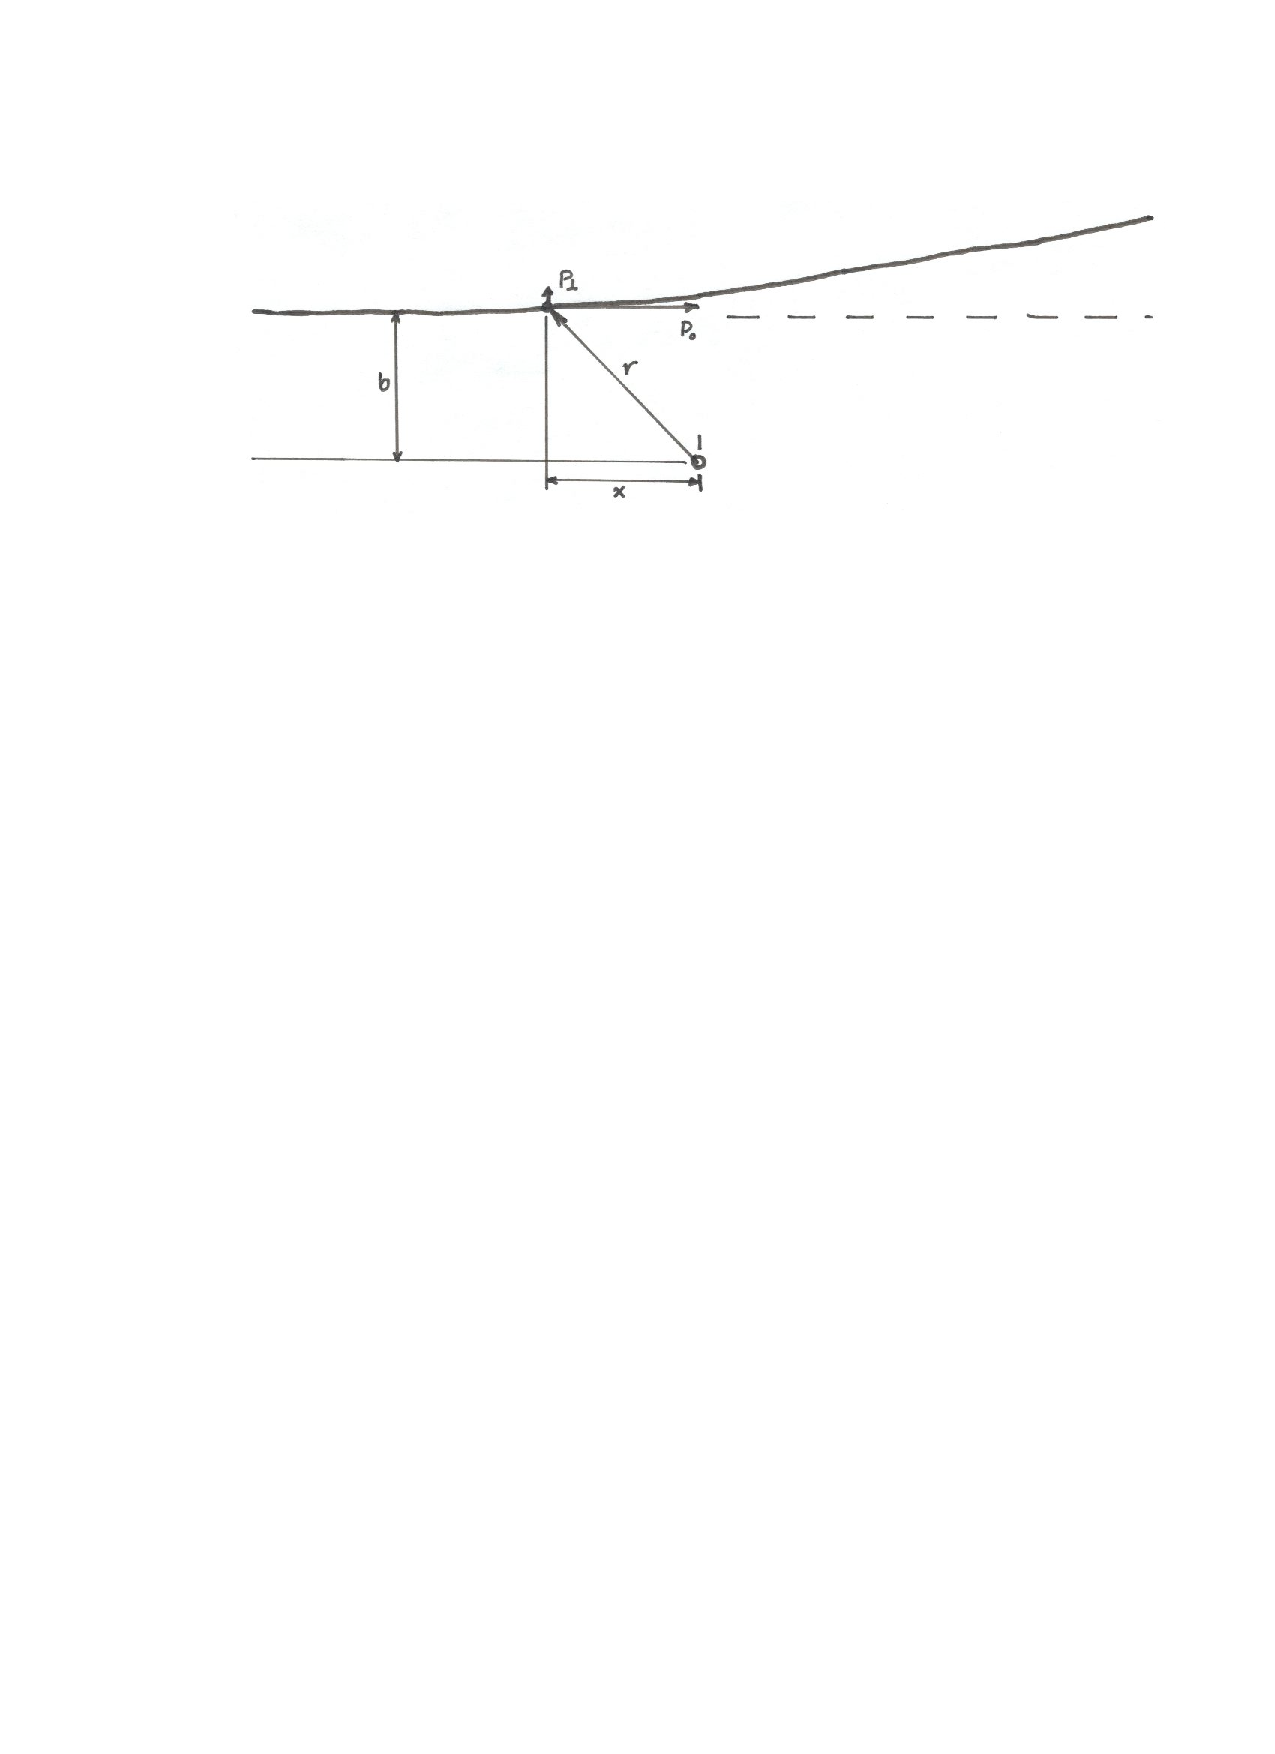
\includegraphics[width=\textwidth]{Figures/scattering}
\caption{Geometry for scattering problem.}
\label{f.scattering}
\end{figure}

As mentioned earlier, we are in a weakly coupled plasma, so we expect large angle scatterings to be a rare occurrence. What happens instead is that the particle suffers a number of small deflections. Let's consider an impact parameter in the range $(b,b+\dif b)$. Each deflection will have $\bvec{\Delta p}_{\bot}$ in some random direction, so
\[ \langle \bvec{ p}_{\bot}\rangle = \sum_{i=1}^{N} \bvec{\Delta p}_{i} \approx \bvec{0}. \]
What is happening is that the component of momentum perpendicular to $p_{0}$ is executing a random walk.  Indeed, after $N$ collisions,
\begin{eqnarray*} \langle \bvec{p}_{\bot} \vdot \bvec{p}_{\bot} \rangle  &=& \left( \sum_{i=1}^{N} \bvec{\Delta p}_{i}\right)\vdot \left( \sum_{i=1}^{N} \bvec{\Delta p}_{i} \right) \\
&=& \sum_{i=1}^{N} (\Delta p_{i})^{2} + 2\sum_{i\ne j} \bvec{\Delta p}_{i}\vdot\bvec{\Delta p}_{j} = N(\Delta p_{\bot})^{2},
\end{eqnarray*}
where we have assumed that all $\bvec{\Delta p}_{\perp}$ have the same magnitude and are uncorrelated. Now $N$ is just $\Delta t \times n \times (2\pi b \,\dif b) \times (p_{0}/\mu)$: the number of particles with impact parameters between $b$ and $b+\dif b$ along the length of the particles path over a time $\Delta t$.  Dividing by $\Delta t$ and integrating over $b$, we have the rate of change of the perpendicular component of the momentum
\begin{equation}\label{e.msdev-momentum}
\frac{\dif \langle p_{\bot}^{2}\rangle }{\dif t} = \frac{8\pi n\mu (q_{1}q_{2})^{2}}{p_{0}}\int_{b_{\mathrm{min}}}^{b_{\mathrm{max}}}\;\frac{\dif b}{b}.
\end{equation}
What are $b_{\mathrm{max}}$ and $b_{\mathrm{min}}$, the maximum and minimum impact parameters? Clearly, if $b > \lambda_{\mathrm{D}}$ then the potential will be screened.  Since our approximation is only good for $b > b_{0}$, we may take $b_{\mathrm{min}} = b_{0}$. (Our rate of scattering only depends logarithmically on $b_{\mathrm{max}}/b_{\mathrm{min}}$, so these estimates are good enough for our purposes).  With this substitution,
\begin{eqnarray}
\frac{\dif \langle p_{\bot}^{2}\rangle }{\dif t} &=& \frac{8\pi n\mu (q_{1}q_{2})^{2}}{p_{0}}\ln\left(\frac{\lambda_{\mathrm{D}}}{b_{0}}\right)\nonumber \\
 &\equiv& \frac{8\pi n\mu (q_{1}q_{2})^{2}}{p_{0}}\ln\Lambda.
\label{e.deflection-rate}
\end{eqnarray}
In the literature, the quantity $\ln\Lambda$ is called the Coulomb logarithm; for a plasma such as we are considering it is $\sim \ln  \left(\Lambda_{\mathrm{D}}^{3} n\right)$, the logarithm of the number of particles in a Debye sphere (see eq.~[\ref{e.plasma-parameter}]).  For conditions typical of the solar center (hydrogen plasma, $\rho \gtrsim 1\nsp\grampercc$, $T \approx 10^{7}\nsp\K$), $\ln\Lambda \approx \left(5\textrm{--}10\right)$.  

For small-angle scattering, the concept of a collision rate is fuzzy: the particle is constantly being bombarded by many tiny collisions.  Setting $\dif \langle p_{\bot}^{2}\rangle/\dif t = p_{0}^{2}\nu$ allows us to define a deflection rate,
\begin{eqnarray}\label{e.scattering-rate}
\nu &\approx& \frac{8\pi n \mu (q_{1}q_{2})^{2}}{p_{0}^{3}} \ln\Lambda\\
 &=& \frac{8\pi n (q_{1}q_{2})^{2}}{(3\kB T)^{3/2}\mu^{1/2}}\ln\Lambda.
\end{eqnarray}
Comparing equations~(\ref{e.scattering-rate}) and (\ref{e.large-angle-collision-rate}), we see that many small angle scatterings are more important than single large angle scattering. Note that the ion-ion collision rate will be about $\sqrt{m_{p}/m_{e}} \approx 43$ times less than the electron-electron collision rate for a given temperature.

One can define a mean free path $\ell$ from equation~(\ref{e.scattering-rate}). Consider a particle incident on a cylinder of cross-sectional area $\mathcal{A}$ and length $\ell$, as illustrated in Figure~\ref{f.mfp}. We chose $\ell$ so that the time for the particle to traverse it is $\nu^{-1}$, the timescale for deflection.  Thus $\ell = v_{0}/\nu = p_{0}/(\mu\nu)$. Note that for a large angle collision, we can write the probability for scattering as the total cross-section of scatterers per unit area,
\begin{equation}\label{e.mfp-simple}
\mathcal{P} = \frac{N\sigma}{\mathcal{A}} = \frac{n\times(\ell\mathcal{A})\sigma}{\mathcal{A}},
\end{equation}
so the particle will suffer on average a collision after traversing a distance $\ell = (n\sigma)^{-1}$. Comparing equation~(\ref{e.mfp-simple}) with our expression for $\ell$ in terms of $\nu$ allows us to define an effective cross-section for small angle scattering.

\begin{marginfigure}
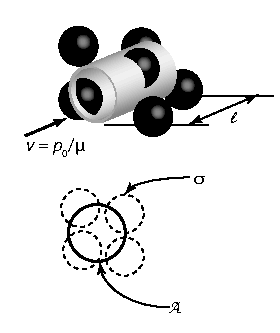
\includegraphics[width=\linewidth]{Figures/mean-free-path}
\caption{Schematic of a particle incident on a cylinder containing $n\times\ell\times\mathcal{A}$ particles.}
\label{f.mfp}
\end{marginfigure}

\section{Transport coefficients}

We now have enough machinery to make estimates of \emph{transport coefficients,} such as the viscosity and the thermal conductivity. Let's begin with the viscosity.  Suppose we have a fluid with a gradient in the velocity, a shear, as depicted in Figure~\ref{f.shear-diagram}.  Let the mean thermal velocity of a particle be $v_{0}$.  In a time $\Delta t$, a number of particles will enter the box from the top, $(1/6) n v_{0} \Delta t$, and a similar number will leave the box via the top face. On average, these particles are endowed with the fluid properties of their last scattering, so the \emph{net} momentum carried into the box across the top face is
\begin{equation}\label{e.viscosity-1}
 \frac{1}{6} n m v_{0} \Delta t \Delta A \left[v_{y}(z_{t} + \ell) - v_{y}(z_{t}-\ell)\right] \approx \frac{1}{3} n m v_{0} \Delta t\Delta A \left.\frac{\partial v_{y}}{\partial z}\right|_{z_{t}}\ell.
\end{equation}
Here $\Delta A$ is the cross-section area of our box in the $xy$ plane and $z_{t}$ is the coordinate of the top face.

\begin{marginfigure}
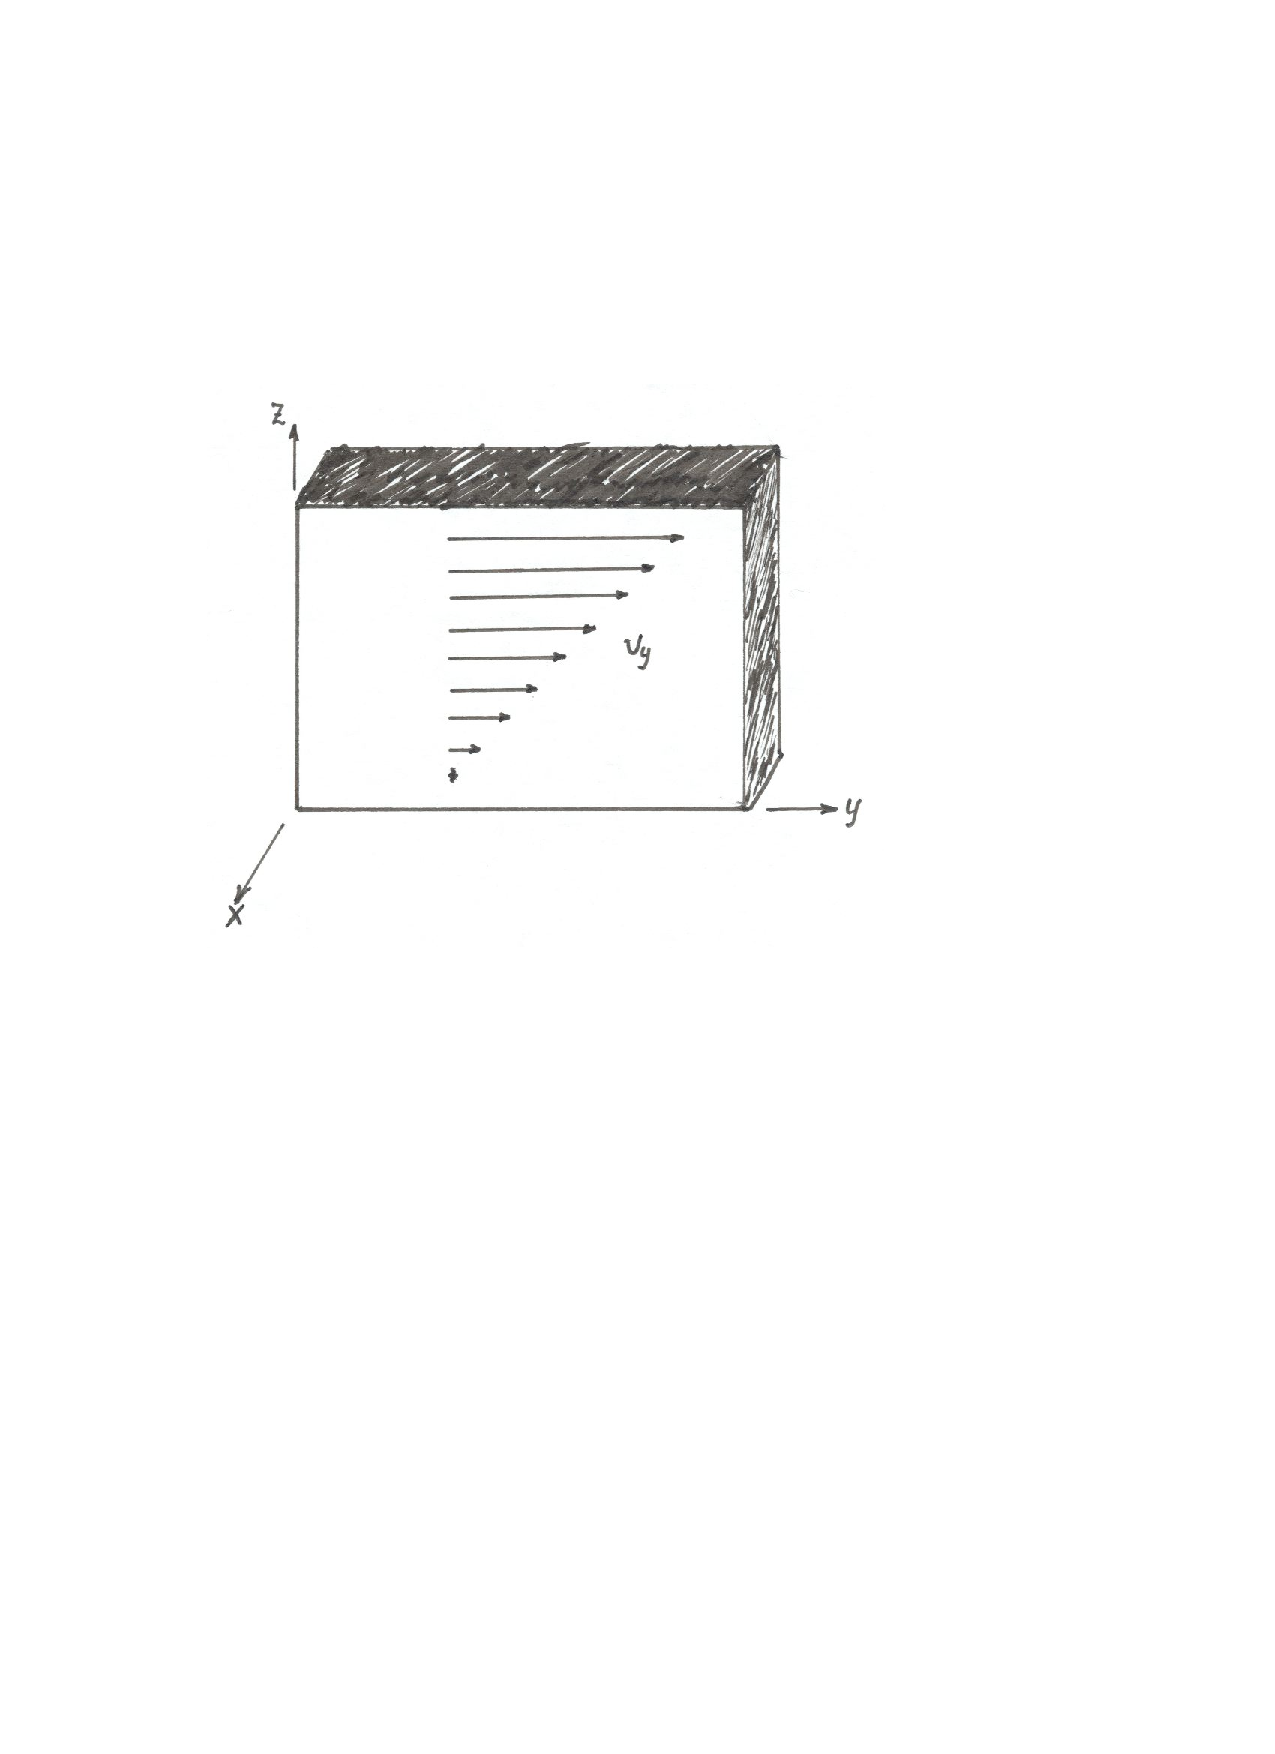
\includegraphics[width=\linewidth]{Figures/shear-diagram}
\caption{An element of fluid with a shear $\partial v_{y}/\partial z$.}\label{f.shear-diagram}
\end{marginfigure}

A similar process occurs across the bottom face, located at coordinate $z=z_{b}$: the momentum flux across the bottom face is
\begin{equation}\label{e.viscosity-2} 
\approx -\frac{1}{3} n m v_{0} \Delta t\Delta A \left.\frac{\partial v_{y}}{\partial z}\right|_{z_{b}}\ell.
\end{equation}
Note the difference in sign: the momentum flux is positive if the $y$-velocity is larger below the box.  Putting equations~(\ref{e.viscosity-1}) and (\ref{e.viscosity-2}) together, the net change of momentum per time per unit volume $\Delta A\Delta z$ is
\begin{eqnarray}
\frac{m}{\Delta A\Delta z}\frac{\Delta v_{y}}{\Delta t} &\approx&  \frac{1}{\Delta z} \frac{1}{3} \left[\left(n m v_{0}\ell\frac{\partial v_{y}}{\partial z}\right)_{z_{t}} - \left(n m v_{0} \ell\frac{\partial v_{y}}{\partial z}\right)_{z_{b}}\right]\nonumber\\
 &\approx&   \frac{\partial}{\partial z}\left( \mu \frac{\partial v_{y}}{\partial z}\right).
\label{e.viscosity-3}
\end{eqnarray}
Here we have defined $\mu = nmv_{0}\ell/3 $ as the coefficient of dynamic viscosity. 

On the left-hand side, the quantity $m/(\Delta A\Delta z)$ is just the mass density $\rho$, and equation~(\ref{e.viscosity-3}), so the left-hand side is the $y$-component of our old friend $\rho(\partial_{t}\vu + \vu\vdot\grad\vu$.  On the right-hand side, we can repeat the above derivation for the transport of momentum in the $x$- and $y$-directions; if we also add back in forces from gravity and pressure gradients, we transform Euler's equation, eq.~(\ref{e.euler}), to the \emph{Navier-Stokes equation},
\begin{equation}\label{e.navier-stokes}
\partial_{t}\vu + \vu\vdot\grad\vu = -\grad \Phi - \frac{1}{\rho}\grad P + \frac{1}{\rho}\divr(\mu \grad\vu).
\end{equation}
In an isothermal, incompressible fluid, one can pull $\mu$ outside the divergence operator and the last term becomes
\[ \frac{\mu}{\rho}\nabla^{2}\vu \equiv \nu \nabla^{2}\vu, \]
where $\nu$ is defined as the \emph{coefficient of kinematic viscosity} (sorry for the overload of notation with the scattering frequency earlier!). Note that in order-of-magnitude
\[ \nu \sim \frac{1}{3}v_{0}\ell,\]
that is, it is roughly the thermal velocity times the mean free path.

An identical proceedure, but replacing the average momentum of a particle with its average thermal energy, yields an expression for the \emph{thermal conductivity} $K$, such that the heat flux is
\begin{equation}\label{e.flux-equation}
\bvec{F} = -K\grad T.
\end{equation}
If one writes the change in energy of a fluid element as being 
\[\rho C \partial_{t}T = \divr(K\grad T),\]
 it can be seen that in order of magnitude the thermal diffusivity $\chi \equiv K/(\rho C)$, where $C$ is the specific heat per unit mass, is $\chi \sim (1/3) v_{0} \ell$.  (From the form of the equation and dimensional analysis, it has to be like this.)  But we need to be careful here: in a plasma with ions and electrons, the ions are responsible for momentum transport, whereas electrons, being more nimble, are more effective at heat transport.  Thus the thermal diffusivity is larger than the kinematic viscosity by a factor $\sim \sqrt{m_{p}/m_{e}}\approx 43$.

\section{Exercises}\label{s.plasma-exercises}
\begin{enumerate}

\item Estimate the ratio of the pressure to viscous accelerations,
\[ \frac{|\rho^{-1}\grad P|}{|\nu\nabla^{2}\vu|} ,\]
in equation~(\ref{e.navier-stokes}).  Express your answer in terms of a characteristic lengthscale, Mach number, and mean free path.  Under what conditions are viscous effects important?

\item Estimate the plasma thermal conductivity under conditions appropriate to the solar center. How does heat conduction by the electrons compare to that by photons?

%\item Estimate the ratio of the conduction heat flux carried by electrons to that carried by photons, at conditions appropriate to the solar center.  For non-degenerate electrons the conductivity is \citep{spitzer62:_physic}
%\[
%K \approx 3.1\ee{12}  \left(\frac{T}{10^{7}\nsp\K}\right)^{5/2}\frac{1}{Z}\nsp\ergs\usp\K^{-1}\nsp\cm^{-1}\nsp\second^{-1}.
%\]
Now suppose we wish to write a single equation for heat transport,
\[
\bvec{F} =  -\frac{4}{3} \frac{acT^{3}}{\rho\kappa_{\mathrm{total}}}\grad T.
 \]
Derive an expression for $\kappa_{\mathrm{total}}$ in terms of the electron conductivity $K$ and the free-free opacity $\kappa_{\mathrm{ff}}$.  

\end{enumerate}
